\chapter{Methods}\label{ch:methods}

\section{Framework Overview}\label{sec:framework}

This chapter describes how we construct and analyze kinetic models of
short peptide sequences based on their underlying \emph{energy landscapes}.
Instead of following long molecular dynamics trajectories directly, we
separate the problem into three complementary layers:

\begin{enumerate}
  \item \textbf{Sampling the energy landscape.} Using the LAMMPS
        implementation of the Mpipi coarse-grained potential, interfaced
        to the global optimization code GMIN (LMPGMIN) and the transition-state
        search code OPTIM (LMPOPTIM), we build for each sequence a large
        database of local minima and transition states following the
        protocol of Nicy \emph{et al.}\ for hexapeptides \cite{Nicy2024Mpipi}.
        Basin-hopping Monte Carlo moves in configuration space, rather
        than time-resolved MD, provide the primary sampling mechanism.

  \item \textbf{Constructing a continuous-time Markov chain.} From these
        stationary points we use harmonic transition state theory (TST),
        as implemented in the Wales-group toolkit PyGT, to assign rate
        constants for transitions between minima. We thus define a
        continuous-time Markov chain: a stochastic process that jumps
        between minima with well-specified rates.

  \item \textbf{Coarse-graining and network analysis.} The microscopic Markov chain
      typically contains $N\sim 10^3$--$10^5$ minima. We apply a graph transformation
      (GT) procedure to eliminate intermediate minima while preserving mean first-passage
      times (MFPTs) between a chosen set of retained states. Spectral quantities
      (eigenvalues and relaxation times) and graph-theoretic distances are computed on
      the reduced generator, where they are numerically stable and interpretable. MFPTs
      computed on the microscopic models serve as the kinetic baseline for validating the
      coarse-grained reductions.
\end{enumerate}

The key advantage of this framework is that it avoids the need for long time-resolved
molecular dynamics trajectories, which can require prohibitively long sampling to
resolve rare barrier-crossing events. By representing the dynamics as a continuous-time
Markov chain on minima, slow kinetic observables such as mean first-passage times can
be computed directly from sparse linear algebra. This separation isolates the physical
input (the potential energy surface and its stationary points) from the probabilistic
analysis, and enables controlled coarse-graining without discarding the long-time
kinetic information used for sequence comparisons in this thesis.

Throughout this chapter we denote the temperature by $T$ and the
inverse temperature by $\beta = 1/(k_{\mathrm{B}}T)$, where
$k_{\mathrm{B}}$ is Boltzmann's constant. Energies are measured in
consistent units (kcal/mol), but the absolute prefactor that
converts dimensionless rates into physical time units is not essential
for the comparative analysis performed in this thesis.

\begin{figure}[ht]
  \centering
  \begin{tikzpicture}[
    node distance=7mm,
    box/.style={
      rectangle,
      rounded corners=3pt,
      draw=black!50,
      fill=black!8,
      line width=0.8pt,
      align=center,
      inner sep=3pt,
      minimum width=4.1cm,
      minimum height=1.0cm,
      font=\small,
      text=black
    },
    arrow/.style={-{Latex[length=3mm]}, thick, color=black!50}
  ]

    % Nodes: vertical pipeline
    \node[box] (seq) {Short peptide\\sequence(s)};
    \node[box, below=of seq] (mpipi) {Mpipi coarse-grained\\potential in LAMMPS\\(energy/force engine)};
    \node[box, below=of mpipi] (sampling) {Basin-hopping \&\\discrete path sampling\\(GMIN/OPTIM)};
    \node[box, below=of sampling] (db) {Stationary-point database\\(\texttt{min.data}, \texttt{ts.data},\\connectivity files)};
    \node[box, below=of db] (ctmc) {Microscopic continuous-time\\Markov chain $Q(T)$ on minima};
    \node[box, below=of ctmc] (gt) {Graph transformation\\to kept minima $\mathcal{K}$};
    \node[box, below=of gt] (analysis) {Coarse-grained kinetics \&\\network analysis\\(MFPTs, relaxation times,\\graph distances)};

    % Layer boxes / labels
    \node[
      draw=black!30,
      dashed,
      rounded corners=3pt,
      line width=0.8pt,
      fit=(mpipi) (sampling) (db),
      inner sep=5pt,
      label=right:{\small\color{black!60} Sampling the energy landscape}
    ] (layer1) {};

    \node[
      draw=black!30,
      dashed,
      rounded corners=3pt,
      line width=0.8pt,
      fit=(ctmc),
      inner sep=5pt,
      label=right:{\small\color{black!60} Continuous-time Markov chain}
    ] (layer2) {};

    \node[
      draw=black!30,
      dashed,
      rounded corners=3pt,
      line width=0.8pt,
      fit=(gt) (analysis),
      inner sep=5pt,
      label=right:{\small\color{black!60} Coarse-graining \& analysis}
    ] (layer3) {};

    % Arrows
    \draw[arrow] (seq) -- (mpipi);
    \draw[arrow] (mpipi) -- (sampling);
    \draw[arrow] (sampling) -- (db);
    \draw[arrow] (db) -- (ctmc);
    \draw[arrow] (ctmc) -- (gt);
    \draw[arrow] (gt) -- (analysis);

  \end{tikzpicture}
  \caption{Overview of the modelling framework used in this thesis. Short peptide sequences are evaluated using the Mpipi coarse-grained potential in LAMMPS, stationary points on the corresponding energy landscape are collected via basin-hopping and discrete path sampling, a microscopic continuous-time Markov chain $Q(T)$ is constructed on the minima, and graph transformation yields a smaller kinetic model on a chosen set of minima for subsequent network and spectral analysis, validated against microscopic MFPT baselines.}
  \label{fig:framework-overview}
\end{figure}


%% ====================================================================
%%  SECTION 2: FROM MOLECULAR CONFIGURATIONS TO ENERGY LANDSCAPES
%% ====================================================================

\section{From Molecular Configurations to Energy Landscapes}\label{sec:method_disconnectivity}

The following procedures follow the protocol established by Nicy and Wales
\cite{Nicy2024Mpipi,Wales2023PeptideTrees}. As the central contributions of this
thesis concern continuous-time Markov chains, coarse-grained kinetics, and network
analysis, we give only a brief overview of how the stationary-point databases and
disconnectivity graphs are generated, and devote greater attention to
Sections~\ref{sec:ktn}--\ref{sec:regression}.

\subsection{Intuitive Picture: Minima, Saddles, and the Hiking Analogy}\label{subsec:intuition}

The \emph{energy landscape} of a peptide is a high-dimensional surface defined over
all possible configurations of its coarse-grained beads. One can picture this landscape
as a rugged mountain range:

\begin{itemize}
  \item Each \textbf{valley} (local minimum) corresponds to a stable or metastable
        structure of the peptide.
  \item Each \textbf{mountain pass} or \textbf{saddle point} (transition state) is
        the lowest route for crossing from one valley to another.
  \item At finite temperature, the peptide behaves like a hiker performing a random
        walk on this terrain, lingering in valleys and occasionally gaining enough
        thermal energy to cross a pass.
\end{itemize}

Our goal is to describe the dynamics in terms of these valleys and passes, rather
than tracking every step of the hiker along the continuous paths in between. Direct
molecular dynamics would literally follow the hiker's footsteps and is often dominated
by long waiting times in deep valleys. Discrete path sampling (DPS) instead focuses on
\emph{where} the hiker can go and \emph{which passes} connect the important valleys,
producing a compact network representation that is much better suited to the kinetic
and network analyses in this thesis.

\subsection{Coarse-Grained Model and LAMMPS Interfaces}\label{subsec:mpipi}

For each six-residue peptide sequence (see Appendix~\ref{ch:sequences} for the full
list), we adopt the Mpipi residue-level coarse-grained potential implemented in LAMMPS
\cite{Thompson2022LAMMPS}, following Nicy \emph{et al.}\ \cite{Nicy2024Mpipi}. Mpipi
represents each amino acid by a single interaction site with sequence-dependent
short-range attractive and electrostatic interactions calibrated to reproduce
single-chain properties and phase behavior of intrinsically disordered proteins
\cite{Joseph2021Mpipi}.

In this work, we do \emph{not} generate long molecular dynamics trajectories.
Instead, LAMMPS is used purely as an energy and force engine for geometry optimization
and transition-state searches, driven by the external codes GMIN and OPTIM:

\begin{itemize}
  \item The LAMMPS--GMIN interface (LMPGMIN) performs basin-hopping global optimization
        of monomers and dimers, exploring low-lying minima.
  \item The LAMMPS--OPTIM interface (LMPOPTIM), coordinated by PATHSAMPLE, performs
        discrete path sampling and builds up the network of transition states connecting
        minima.
\end{itemize}

All Mpipi parameters (bonded terms, non-bonded interactions, electrostatics, and
cutoffs) and the LAMMPS input files follow those used in Nicy \emph{et al.}\
\cite{Nicy2024Mpipi}. Our goal in this first layer is to replicate and extend their
energy-landscape databases for use in kinetic and network analysis.

\subsection{Global Optimization by Basin-Hopping}\label{subsec:basin-hopping}

For each sequence, we first obtain a representative set of low-lying minima using
basin-hopping global optimization in GMIN with the LAMMPS interface
\cite{Wales1997BasinHopping,Nicy2024Mpipi}. Basin-hopping can again be understood in
hiking language: we repeatedly ``kick'' the hiker to a new trial location, slide them
downhill until they reach the bottom of the nearest valley, and then decide whether to
keep this new valley or stay in the old one.

Concretely, from a current minimum we propose a structural perturbation (Cartesian moves
for monomers, plus occasional rigid-body moves for dimers), minimize the perturbed
structure using L-BFGS, and apply a Metropolis acceptance test at a basin-hopping
temperature. Because the acceptance/rejection decision is taken \emph{after} minimization,
the algorithm produces a Monte Carlo walk over minima, not a faithful real-time trajectory.

The purpose of this stage is purely exploratory. We attempt to discover the global
minimum and a large collection of low-energy competitors without running long time
simulations. We run multiple basin-hopping trajectories with different seeds and move
parameters until convergence criteria similar to those of Nicy \emph{et al.}\ are met
\cite{Nicy2024Mpipi}. The output is a set of minimized structures and their energies,
which become the starting points for DPS.

\subsection{Discrete Path Sampling and Stationary-Point Databases}\label{subsec:dps}

To convert the set of minima into a connected kinetic transition network, we employ
discrete path sampling (DPS) using OPTIM interfaced to LAMMPS, with PATHSAMPLE as the
driver code \cite{Wales2002DPS,Wales2003Book,Nicy2024Mpipi}. DPS repeatedly chooses
pairs of minima that appear important or insufficiently connected, searches for
transition states connecting them, and expands the database until the main low-energy
regions of the landscape are well linked.

The search combines several standard ingredients from the Wales group methodology:
doubly-nudged elastic band (DNEB) calculations to propose minimum-energy paths
\cite{Trygubenko2004DNEB}, hybrid eigenvector-following to refine first-order saddle
points \cite{Munro1999HEF}, steepest-descent connections from each saddle down to its
endpoint minima, and ``missing-connection'' and distance-based heuristics to identify
promising pairs of minima that are close in energy or structure but not yet connected
\cite{Roder2018Abeta}.

As DPS iterates, it accumulates for each sequence a \emph{stationary-point database}
consisting of:

\begin{itemize}
  \item a list of minima (\texttt{min.data}) with their energies and vibrational data,
  \item a list of transition states (\texttt{ts.data}) with energies and indices of the
        two minima each saddle connects,
  \item index files (\texttt{points.min}, \texttt{points.ts}) of the main connected
        component of the network,
  \item optional labels (\texttt{min.A}, \texttt{min.B}) marking reactant- and
        product-like sets of minima for later mean first-passage time calculations.
\end{itemize}

These files mirror the DPS outputs in Nicy \emph{et al.}\ \cite{Nicy2024Mpipi}. In
this thesis, all subsequent Markov modelling, graph transformation, and network
analysis use only this stationary-point database as input.

\subsection{Disconnectivity Graphs}\label{subsec:disconnectivity}

Before constructing kinetic models, we visualize each sequence's energy landscape
using \emph{disconnectivity graphs} generated by PATHSAMPLE
\cite{Wales1998Archetypal}. In a disconnectivity graph, minima are plotted according
to their energies on the vertical axis (lower is more stable), branches show how
basins merge as the energy threshold is raised, and the overall branching pattern
reveals single-funnel versus multi-funnel topologies and the degree of frustration.

A disconnectivity graph gives us an immediate visual sense of whether a sequence has
one dominant funnel or several competing funnels separated by large barriers. In this
thesis, we use these graphs both to verify that we reproduce the landscapes reported by
Nicy \emph{et al.}\ and to guide the choice of ``important'' minima to retain in
coarse-grained kinetic models (e.g., the lowest minima in each major basin).

This section therefore completes the data-generation layer of the thesis: starting from
sequences and the Mpipi model, we obtain stationary-point databases and disconnectivity
graphs for each monomer and dimer, following Nicy \emph{et al.}, and use these as the
inputs for the kinetic and network analyses that follow.

\begin{figure}[ht]
  \centering
  \hspace*{-0.5cm}%
  \begin{tikzpicture}[
    every node/.style={font=\scriptsize},
    node distance = 6mm and 14mm,
    box/.style={
      rectangle,
      rounded corners=3pt,
      draw=black!50,
      fill=black!8,
      line width=0.8pt,
      align=center,
      inner sep=3pt,
      minimum width=3.8cm,
      minimum height=0.6cm,
      text=black
    },
    group/.style={
      rounded corners=3pt,
      draw=black!30,
      dotted,
      line width=0.8pt,
      inner sep=6pt
    },
    arrow/.style={-{Latex[length=2.5mm]}, thick, color=black!50}
  ]

    %------------- top: sequence + model -------------%
    \node[box] (seq) {Hexapeptide sequence};
    \node[box, below=of seq] (model) {Mpipi model\\\& LAMMPS input};

    %------------- left branch: basin hopping -------------%
    \node[box, below left=0.3cm and 1.3cm of model] (bh)
      {Basin-hopping\\(GMIN / LMPGMIN)};
    \node[box, below=of bh] (minima)
      {Low-lying minima\\(energies \& geometries)};

    %------------- right branch: DPS -------------%
    \node[box, below right=0.5cm and 1.6cm of model, yshift = 0.5cm] (dpssetup)
      {DPS setup:\\seed pairs \&\\control files};
    \node[box, below=of dpssetup, yshift = 0.4cm] (ts)
      {Transition states \&\\connectivity\\(OPTIM / LMPOPTIM\\+ PATHSAMPLE)};

    %------------- grey grouping boxes -------------%
    \node[group, fit=(bh)(minima)] (bhgroup) {};
    \node[group, fit=(dpssetup)(ts)] (dpsgroup) {};

    % labels above groups
    \node[font=\scriptsize, black!50, above=2mm of bhgroup] {Global optimization};
    \node[font=\scriptsize, black!50, above=2mm of dpsgroup] {Discrete path sampling};

    %------------- recombine in the middle -------------%
    \node[box, below=12mm of $(minima)!0.5!(ts)$] (db)
      {Stationary-point database\\
       \scriptsize(\texttt{min.data}, \texttt{ts.data}, \texttt{points.min/ts}, \texttt{min.A/B})};

    \node[box, below=of db] (disc)
      {Disconnectivity graphs\\for each sequence};

    %------------- arrows -------------%
    \draw[arrow] (seq) -- (model);
    \draw[arrow] (model.west) -- (bhgroup.north east);
    \draw[arrow] (model.east) -- (dpsgroup.north west);
    \draw[arrow] (bh) -- (minima);
    \draw[arrow] (dpssetup) -- (ts);
    \draw[arrow, looseness=0.7]
      (minima.south west) to[out=210,in=150] node[left,pos=0.5]{iterate} (bh.north west);
    \draw[arrow, looseness=0.7]
      (ts.south east) to[out=-30,in=30] node[right,pos=0.5]{iterate} (dpssetup.north east);
    \draw[arrow] (bhgroup.south) |- (db.west);
    \draw[arrow] (dpsgroup.south) |- (db.east);
    \draw[arrow] (db) -- (disc);

  \end{tikzpicture}
  \caption{Data-generation pipeline for this thesis. For each hexapeptide
  sequence, the Mpipi model and LAMMPS input files define the underlying
  energy function. Basin-hopping (GMIN / LMPGMIN) produces low-lying
  minima, while discrete path sampling (OPTIM / LMPOPTIM with PATHSAMPLE)
  supplies transition states and connectivity. These ingredients form a
  stationary-point database, which is summarised as disconnectivity
  graphs characterizing the energy landscape of each sequence
  \cite{Wales1998Archetypal,Nicy2024Mpipi}.}
  \label{fig:data-generation-disconnectivity}
\end{figure}


%% ====================================================================
%%  SECTION 3: FROM STATIONARY POINTS TO CTMC
%% ====================================================================

\section{From Stationary Points to a Continuous-Time Markov Chain}\label{sec:ktn}

Once we have a stationary-point database for a given sequence, we turn
it into a kinetic model. The core idea is to approximate the peptide
dynamics as a continuous-time Markov chain on the set of minima
$\mathcal{M} = \{1,\dots,N\}$:

\begin{itemize}
  \item When the system is in minimum $j$, it waits for a random amount
        of time (exponentially distributed) with mean $\tau_j$.
  \item It then jumps to a neighboring minimum $i$ with probability
        $B_{ij}$, where $B$ is a branching probability matrix derived
        from TST rates.
\end{itemize}

Figure~\ref{fig:landscape-to-ktn} illustrates how minima and transition states on
the energy landscape are converted into a discrete kinetic network. We now describe
the ingredients of this Markov chain in detail.

\subsection{Harmonic Approximation and Local Partition Functions}\label{subsec:harmonic}

Near a local minimum $i$, the potential energy can be approximated by a
quadratic (harmonic) expansion:
\begin{equation}\label{eq:harmonic-expansion}
  V(\mathbf{x}) \approx E_i + \frac{1}{2} \sum_{k=1}^{f}
  \lambda_{i,k}\, q_{i,k}^2,
\end{equation}
where $E_i$ is the energy at the minimum, $q_{i,k}$ are normal-mode coordinates,
$\lambda_{i,k}$ are the corresponding eigenvalues (curvatures), and $f$ is the number
of vibrational degrees of freedom (total degrees of freedom minus overall translations
and rotations).

In the harmonic approximation, the local partition function associated
with minimum $i$ at temperature $T$ is, up to a global constant,
\begin{equation}\label{eq:Zi}
  Z_i(T) \;\propto\;
  \frac{\exp(-\beta E_i)}{\prod_{k=1}^{f} \nu_{i,k}},
\end{equation}
where $\nu_{i,k}$ are the vibrational frequencies. In practice,
PATHSAMPLE does not store each $\nu_{i,k}$ separately; instead it stores
the \emph{log-product}
\begin{equation}
  \ln \Pi_i \equiv \ln \left( \prod_{k=1}^{f} \nu_{i,k} \right),
\end{equation}
which suffices for all ratio calculations.

The equilibrium occupation probability of minimum $i$ in the harmonic
superposition approximation is then
\begin{equation}\label{eq:pi-eq}
  \pi_i(T) \;=\;
  \frac{Z_i(T)}{\displaystyle \sum_{j\in\mathcal{M}} Z_j(T)}.
\end{equation}
Intuitively, $\pi_i$ tells us what fraction of the time the system
would spend in minimum $i$ if we could sample configuration space
exhaustively, under the harmonic approximation.

In implementation, we do not compute $Z_i(T)$ explicitly. Instead, the
PyGT toolkit takes the stored energies and vibrational log-products
from \texttt{min.data} and constructs $\pi_i$ internally through a
log-sum-exp procedure that avoids numerical underflow.


\subsection{Harmonic Transition State Theory Rates}\label{subsec:htst}

Next, we assign rate constants $k_{i\leftarrow j}(T)$ for transitions
between minima. Consider a transition state $\alpha$ that connects
minima $i$ and $j$. Let $E_\alpha^\ddagger$ denote its energy and
$\Pi_\alpha^\ddagger$ the product of its positive vibrational frequencies
(there are $f-1$ of these, because one direction is unstable along the
reaction coordinate).

Harmonic transition state theory (TST) gives the rate for the transition
$j \to i$ via saddle $\alpha$ as
\begin{equation}\label{eq:htst-rate}
  k^{(\alpha)}_{i\leftarrow j}(T)
  \;=\;
  \kappa(T)\,
  \exp\!\left[-\beta\left(E^\ddagger_\alpha - E_j\right)\right]\,
  \frac{\displaystyle \prod_{k=1}^{f} \nu_{j,k}}
       {\displaystyle \prod_{k=1}^{f-1} \nu^\ddagger_{\alpha,k}},
\end{equation}
where $\kappa(T)$ is a prefactor with units of frequency, typically proportional
to $k_{\mathrm{B}}T/h$, and the exponential factor
$\exp[-\beta(E^\ddagger_\alpha - E_j)]$ penalizes high activation barriers.

Several aspects of this equation deserve emphasis. The exponential Boltzmann factor
encodes the energetic cost of reaching the barrier top: a modest increase in barrier
height can suppress the transition rate by many orders of magnitude. The frequency-product
ratio accounts for entropic differences between the minimum and the transition state:
the numerator represents the density of states at the minimum, while the denominator
represents it at the saddle. When all minima have similar entropic structure, the
prefactor varies slowly and the rates are dominated by the exponential term. For a
set of transitions with varying barriers and frequencies, the prefactor can modulate
rates by factors of 2--10 or more.

Using the log-product notation, we can rewrite Eq.~\eqref{eq:htst-rate} as
\begin{equation}\label{eq:htst-log}
  k^{(\alpha)}_{i\leftarrow j}(T)
  \;=\;
  \kappa(T)\,
  \exp\!\left[
      -\beta\left(E^\ddagger_\alpha - E_j\right)
      + \ln \Pi_j - \ln \Pi^\ddagger_\alpha
  \right].
\end{equation}
All quantities in Eq.~\eqref{eq:htst-log} (energies and log-products of
frequencies) are already collected in the stationary-point database. The common
prefactor $\kappa(T)$ sets the overall time scale but cancels from all
\emph{relative} kinetic comparisons made in this thesis.

If there are multiple transition states connecting the same pair of minima, their
rates are summed:
\begin{equation}\label{eq:kij-sum}
  k_{i\leftarrow j}(T)
  \;=\;
  \sum_{\alpha \in \mathcal{S}(j\to i)} k^{(\alpha)}_{i\leftarrow j}(T),
\end{equation}
where $\mathcal{S}(j\to i)$ denotes the set of transition states in the
forward direction from $j$ to $i$.

In practice, we do not evaluate these expressions manually. Instead, the
PyGT function \texttt{load\_ktn} reads \texttt{min.data},
\texttt{ts.data}, and associated PATHSAMPLE files, and returns the total
rate constants $k_{i\leftarrow j}(T)$ in a sparse matrix form.


\subsection{Branching Probabilities and Waiting Times}\label{subsec:branching}

From the transition rate constants, two derived kinetic quantities characterize the
dynamics on the network. The \emph{total escape rate} from minimum $j$ is
\begin{equation}\label{eq:escape-rate}
  \lambda_j(T) \;=\; \sum_{i\neq j} k_{i\leftarrow j}(T).
\end{equation}
Intuitively, $\lambda_j(T)$ is the expected number of jumps per unit time out of
minimum $j$. The \emph{waiting time} (or mean residence time) at minimum $j$ is the
reciprocal of the escape rate:
\begin{equation}\label{eq:tau}
  \tau_j(T) = \frac{1}{\lambda_j(T)} = \left( \sum_{i\neq j} k_{i\leftarrow j}(T) \right)^{-1}.
\end{equation}

The \emph{branching probability} gives the conditional probability that, upon leaving
$j$, the system jumps to a neighboring minimum $i$:
\begin{equation}\label{eq:branching-prob}
  B_{i\leftarrow j}(T)
  \;=\;
  \frac{k_{i\leftarrow j}(T)}{\lambda_j(T)}.
\end{equation}
For each column $j$, the probabilities sum to one: $\sum_{i\neq j} B_{i\leftarrow j} = 1$.

The pair $(B,\boldsymbol{\tau})$ therefore completely specifies the random-jump process
on the minima: when in $j$, we wait for an exponentially distributed time with mean
$\tau_j$ and then move to $i$ with probability $B_{i\leftarrow j}$. This decomposition
into a ``wait, then jump'' picture is both intuitive and computationally useful, because
it separates the question of \emph{how long} the system stays in a state from the
question of \emph{where} it goes next.


\subsection{The Generator Matrix and Stationary Distribution}\label{subsec:generator}

To connect with standard Markov chain theory, we assemble the rates into
a continuous-time generator matrix $Q(T)$ on $\mathcal{M}$:
\begin{equation}\label{eq:Q-def}
  Q_{ij}(T) \;=\;
  \begin{cases}
    k_{i\leftarrow j}(T), & i\neq j,\\[4pt]
    -\displaystyle\sum_{m\neq j} k_{m\leftarrow j}(T), & i = j.
  \end{cases}
\end{equation}

The diagonal entries $Q_{jj} = -\lambda_j$ are negative, and by construction each
column of $Q$ sums to zero:
\begin{equation}\label{eq:generator-colsum}
  \sum_{i=1}^{N} Q_{ij}(T) = 0 \qquad \text{for all } j.
\end{equation}

This column-sum property ensures conservation of probability: the total probability
flowing out of any state equals the total flowing in. The time evolution of the
probability vector $\mathbf{p}(t) = (p_1(t), \ldots, p_N(t))^\top$ is governed by the
master equation:
\begin{equation}\label{eq:master}
  \frac{d\mathbf{p}(t)}{dt} = Q(T)\,\mathbf{p}(t).
\end{equation}

The \emph{stationary distribution} $\boldsymbol{\pi}(T)$ is the unique probability
vector satisfying
\begin{equation}\label{eq:stationary-dist}
  Q(T)\,\boldsymbol{\pi}(T) = \mathbf{0}, \quad
  \sum_j \pi_j(T) = 1, \quad \pi_j(T) \ge 0.
\end{equation}

For the harmonic TST rates defined above, the stationary distribution takes a
Boltzmann-like form. In the harmonic approximation, the equilibrium population of
minimum $j$ is proportional to
\begin{equation}\label{eq:stationary-dist-explicit}
  \pi_j(T) \;\propto\; \frac{\exp\bigl[-\beta E_j\bigr]}
  {\prod_{\alpha=1}^{f} \nu_\alpha^{(j)}},
\end{equation}
reflecting the interplay between energetic depth (the Boltzmann factor favors
low-energy minima) and entropic breadth (broad basins with many available
configurations are favored by the frequency product in the denominator).

For harmonic TST rates, the generator satisfies \emph{detailed balance}:
\begin{equation}\label{eq:detailed-balance}
  \pi_j(T)\, k_{i\leftarrow j}(T) = \pi_i(T)\, k_{j\leftarrow i}(T),
  \qquad \forall\, i,j.
\end{equation}
This implies that the generator is similar to a real symmetric matrix and therefore
has a complete set of real eigenvalues, with one eigenvalue exactly equal to $0$ and
all others strictly negative.


\subsection{Kinetic Transition Networks}\label{subsec:ktn-defn}

A \emph{kinetic transition network} (KTN) is the weighted directed graph whose nodes
are the minima and whose edge weights are the transition rates $k_{i\leftarrow j}$.
Equivalently, it is the continuous-time Markov chain defined by the generator matrix
$Q$.

The KTN framework is closely related to, but distinct from, Markov state models (MSMs)
commonly used in the molecular dynamics community \cite{Pande2010MSMReview,Noe2013MSMReview}.
MSMs are typically constructed from long molecular dynamics trajectories: frames are
clustered into metastable states, and transition probabilities are estimated from observed
counts of transitions between clusters. KTNs, by contrast, are built directly from
stationary-point databases without requiring trajectory data. Both approaches yield a
Markov model whose properties (equilibrium populations, relaxation timescales, mean
first-passage times) can be computed from the spectrum and structure of the generator,
but the data source and construction methodology differ substantially.

In our implementation, we use PyGT to compute $(B,\boldsymbol{\tau})$ and then
construct $Q(T)$ as
\begin{equation}\label{eq:Q-construction}
  Q(T) = K(T) - \Lambda(T),
\end{equation}
where $K(T)$ is the off-diagonal rate matrix with entries $K_{ij} = k_{i\leftarrow j}$
for $i\neq j$ and $K_{jj} = 0$, and $\Lambda(T)$ is a diagonal matrix with entries
$\Lambda_{jj} = \lambda_j = 1/\tau_j$. For each sequence and temperature, the
microscopic model is stored as sparse matrices and NumPy arrays: the generator
$Q(T)$, branching probabilities $B(T)$, rate matrix $K(T)$, waiting times
$\boldsymbol{\tau}(T)$, and stationary distribution $\boldsymbol{\pi}(T)$.

\begin{figure}[ht]
  \centering
  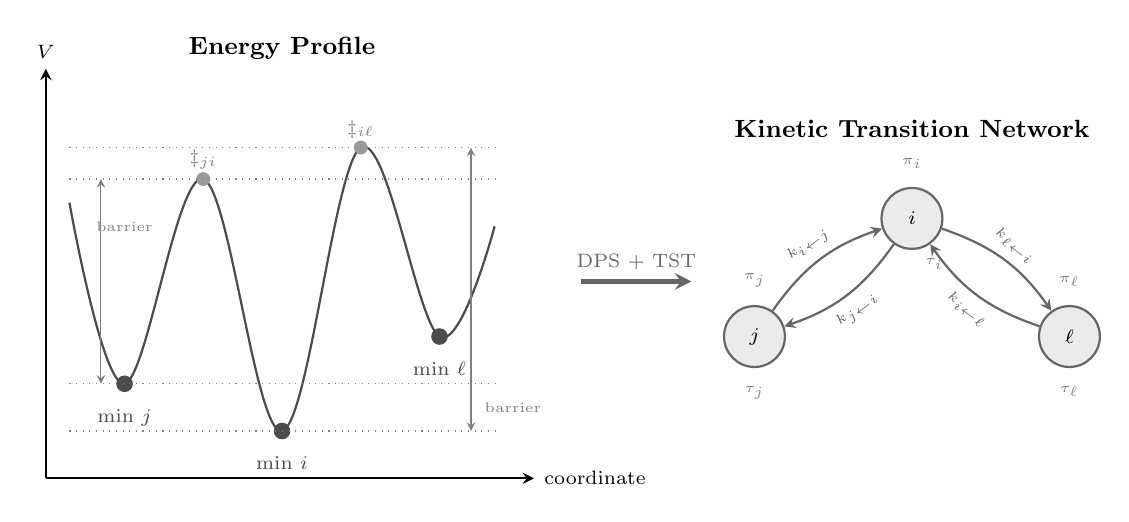
\begin{tikzpicture}[>=stealth, font=\small]
    % --- Left panel: Energy Profile ---
    \begin{scope}[xshift=0cm]
      \node[font=\small\bfseries, anchor=south] at (3, 5.2) {Energy Profile};
      \draw[->, thick] (0, 0) -- (6.2, 0) node[right] {\scriptsize coordinate};
      \draw[->, thick] (0, 0) -- (0, 5.2) node[above] {\scriptsize $V$};

      % Landscape curve
      \draw[thick, black!70]
        plot[smooth, tension=0.6] coordinates {
          (0.3, 3.5) (1.0, 1.2) (2.0, 3.8) (3.0, 0.6) (4.0, 4.2) (5.0, 1.8) (5.7, 3.2)
        };

      % Minima
      \fill[black!70] (1.0, 1.2) circle (3pt);
      \node[below, font=\scriptsize, black!70] at (1.0, 1.0) {min $j$};
      \fill[black!70] (3.0, 0.6) circle (3pt);
      \node[below, font=\scriptsize, black!70] at (3.0, 0.4) {min $i$};
      \fill[black!70] (5.0, 1.8) circle (3pt);
      \node[below, font=\scriptsize, black!70] at (5.0, 1.6) {min $\ell$};

      % Transition states
      \fill[black!40] (2.0, 3.8) circle (2.5pt);
      \node[above, font=\scriptsize, black!50] at (2.0, 3.8) {$\ddagger_{ji}$};
      \fill[black!40] (4.0, 4.2) circle (2.5pt);
      \node[above, font=\scriptsize, black!50] at (4.0, 4.2) {$\ddagger_{i\ell}$};

      % --- Barrier 1: min j to TS ji ---
      \draw[dotted, gray, thin] (0.3, 1.2) -- (5.7, 1.2);
      \draw[dotted, gray, thin] (0.3, 3.8) -- (5.7, 3.8);
      \draw[<->, gray, thin] (0.7, 1.2) -- (0.7, 3.8);
      \node[font=\tiny, gray, anchor=east] at (1.48, 3.2) {barrier};

      % --- Barrier 2: min i to TS il ---
      \draw[dotted, gray, thin] (0.3, 0.6) -- (5.7, 0.6);
      \draw[dotted, gray, thin] (0.3, 4.2) -- (5.7, 4.2);
      \draw[<->, gray, thin] (5.4, 0.6) -- (5.4, 4.2);
      \node[font=\tiny, gray, anchor=west] at (5.45, 0.9) {barrier};
    \end{scope}

    % --- Arrow between panels ---
    \draw[->, ultra thick, black!60] (6.8, 2.5) -- (8.2, 2.5)
      node[midway, above, font=\scriptsize] {DPS + TST};

    % --- Right panel: KTN ---
    \begin{scope}[xshift=9cm, yshift=-0.7cm]
      \node[font=\small\bfseries, anchor=south] at (2.0, 4.9) {Kinetic Transition Network};

      \node[circle, draw=black!60, fill=black!8, thick,
            minimum size=22pt, font=\scriptsize] (j) at (0, 2.5) {$j$};
      \node[circle, draw=black!60, fill=black!8, thick,
            minimum size=22pt, font=\scriptsize] (i) at (2, 4) {$i$};
      \node[circle, draw=black!60, fill=black!8, thick,
            minimum size=22pt, font=\scriptsize] (l) at (4, 2.5) {$\ell$};

      \draw[->, thick, black!60, bend left=18]
        (j) to node[above, font=\tiny, sloped] {$k_{i \leftarrow j}$} (i);
      \draw[->, thick, black!60, bend left=18]
        (i) to node[below, font=\tiny, sloped] {$k_{j \leftarrow i}$} (j);
      \draw[->, thick, black!60, bend left=18]
        (i) to node[above, font=\tiny, sloped] {$k_{\ell \leftarrow i}$} (l);
      \draw[->, thick, black!60, bend left=18]
        (l) to node[below, font=\tiny, sloped] {$k_{i \leftarrow \ell}$} (i);

      \node[font=\tiny, gray, below=3pt] at (j.south) {$\tau_j$};
      \node[font=\tiny, gray, below=3pt] at (i.south east) {$\tau_i$};
      \node[font=\tiny, gray, below=3pt] at (l.south) {$\tau_\ell$};
      \node[font=\tiny, gray, above=3pt] at (j.north) {$\pi_j$};
      \node[font=\tiny, gray, above=3pt] at (i.north) {$\pi_i$};
      \node[font=\tiny, gray, above=3pt] at (l.north) {$\pi_\ell$};
    \end{scope}
  \end{tikzpicture}
  \caption{Construction of a kinetic transition network (KTN) from an energy landscape. Left: a schematic one-dimensional potential energy profile with three local minima connected by two transition states, with both barrier heights annotated by grey dotted lines. Discrete path sampling locates these stationary points, and harmonic transition state theory assigns a rate constant to each directed transition. Right: the resulting KTN, in which each minimum becomes a node carrying a waiting time $\tau$ and equilibrium population $\pi$, and each transition state generates a pair of directed edges with rate constants $k_{i \leftarrow j}$.}
  \label{fig:landscape-to-ktn}
\end{figure}


%% ====================================================================
%%  SECTION 4: KEY KINETIC OBSERVABLES
%% ====================================================================

\section{Key Kinetic Observables}\label{sec:observables}

\subsection{Mean First-Passage Times}\label{subsec:mfpt}

The \emph{mean first-passage time} (MFPT) from a set of states $A$ to a set of
states $B$ is the expected time for a system starting in the equilibrium distribution
on $A$ to reach $B$ for the first time.

Let $m_j$ denote the MFPT from state $j$ (where $j \notin B$) to the target set $B$.
These satisfy a system of linear equations derived from the generator:
\begin{equation}\label{eq:mfpt-linear-system}
  \sum_{i=1}^{N} Q_{ij}\, m_i \;=\; -1, \qquad j \notin B,
\end{equation}
with the boundary condition $m_j = 0$ for all $j \in B$. This is a system of
$|S \setminus B|$ linear equations in $|S \setminus B|$ unknowns.

The MFPT from a set of source states $A$ to a target set $B$ is then the
equilibrium-weighted average of the individual MFPTs:
\begin{equation}\label{eq:mfpt-AB}
  \mathrm{MFPT}(A \to B)
  \;=\;
  \frac{\sum_{j \in A} \pi_j\, m_j}{\sum_{j \in A} \pi_j}.
\end{equation}

In the hexapeptide context, MFPTs between reactant-like and product-like basins
quantify the timescale of structural transitions. A large MFPT indicates that the two
basins are separated by a substantial free-energy or kinetic barrier, making
transitions rare. A small MFPT reflects rapid interconversion. Although these MFPTs
do not represent nucleation rates in an LLPS droplet, they capture the intrinsic
kinetic tendencies of a sequence, including its propensity to become trapped, to
transition between basins, or to access alternative conformational funnels, which are
sequence-dependent determinants relevant to LLPS behavior and aggregation propensity.

MFPTs were computed using PyGT first-passage routines. In the dataset, the reference
sets $A$ and $B$ are singleton microstates for all sequences, so MFPTs and their
variances were obtained using \texttt{compute\_passage\_stats} applied to the full
generator $Q(T)$. When $A$ and/or $B$ contain multiple states, we instead use
\texttt{compute\_rates}, which returns MFPTs together with phenomenological rate
constants. Because graph transformation preserves MFPTs between kept states, the
coarse-grained quantities should be equal to what we would obtain from the full
microscopic model, up to numerical error, but are far cheaper to compute and interpret.


\subsection{Relaxation Times and Spectral Decomposition}\label{subsec:relaxation}

The relaxation times of the system are determined by the eigenvalues of the generator
$Q$. Let $\lambda_1, \lambda_2, \ldots, \lambda_N$ denote the eigenvalues ordered so
that
\begin{equation}\label{eq:eigenvalue-ordering}
  0 = \lambda_1 > \mathrm{Re}(\lambda_2) \geq \mathrm{Re}(\lambda_3) \geq \cdots.
\end{equation}

For a reversible continuous-time Markov chain satisfying detailed balance, all nonzero
eigenvalues are real and negative. The $k$-th relaxation time is defined as
\begin{equation}\label{eq:relaxation-time}
  t_k \;=\; \frac{-1}{\lambda_k}, \quad k \geq 2.
\end{equation}

The time evolution of the probability distribution can be written as a spectral
expansion:
\begin{equation}\label{eq:spectral-decomposition}
  \mathbf{p}(t)
  \;=\;
  \boldsymbol{\pi}
  \;+\;
  \sum_{k=2}^{N} c_k\, e^{\lambda_k t}\, \mathbf{v}_k,
\end{equation}
where $\mathbf{v}_k$ are the right eigenvectors of $Q$ and the coefficients $c_k$
depend on the initial conditions. Each exponential term decays on a timescale
$t_k = -1/\lambda_k$. After a time much longer than $t_2$, all exponentials have
decayed and the system has reached the stationary distribution $\boldsymbol{\pi}$.

The slowest relaxation time $t_2$ sets the overall timescale for equilibration.
A large separation between $t_2$ and higher relaxation times ($t_3, t_4, \ldots$)
indicates a single dominant slow process well-separated from faster modes, suggesting a
landscape with one principal rate-limiting barrier. A ratio $t_2/t_3$ close to one
indicates that multiple slow processes compete on similar timescales, which is a
hallmark of multi-funnel landscapes with several comparably high barriers.

\subsubsection{Why microscopic eigenvalues are not used}

Although detailed balance implies that the microscopic generator is similar to a
symmetric matrix (and therefore has a real spectrum), the fine-grained models in this
thesis can reach $N\sim 10^5$ states. We therefore do not use eigenvalue computations
of the full microscopic generator as a primary diagnostic. Instead, microscopic
validation is performed via sign and conservation checks and the stationarity condition
$Q(T)\boldsymbol{\pi}(T)=\mathbf{0}$. Eigenvalues and relaxation times are computed
only after coarse-graining, on the reduced generator $Q^{\mathrm{eff}}(T)$, where
sparse eigenvalue solvers can reliably estimate the leading eigenvalues.


%% ====================================================================
%%  SECTION 5: COARSE-GRAINING VIA GRAPH TRANSFORMATION
%% ====================================================================

\section{Coarse-Graining via Graph Transformation}\label{sec:gt}

\subsection{Motivation for Coarse-Graining}\label{subsec:cg-motivation}

The microscopic Markov model described above typically contains
$N = \mathcal{O}(10^3\text{--}10^5)$ minima, which is both computationally demanding
and difficult to interpret. For many questions, however, we do not need such fine
resolution. Instead, we care primarily about a small number of \emph{basins} or
\emph{macrostates} (reactant-like, product-like, and key intermediates) and kinetic
observables such as mean first-passage times between these basins.

To focus on this coarse description, we compress the microscopic model into a smaller
Markov chain that keeps a chosen set of important minima as explicit states and
mathematically integrates out all other minima while preserving MFPTs between the kept
states. This procedure is known as \emph{graph transformation} (GT)
\cite{Trygubenko2006GT,Stevenson2014GT,Wales2024FPT}.


\subsection{Selecting Retained Minima}\label{subsec:keep-selection}

Graph transformation requires specification of a set of retained states
$\mathcal{K} \subset \mathcal{M}$. Because MFPT preservation holds for any fixed
$\mathcal{K}$, the key modelling choice is \emph{which} minima should remain explicit.
In this thesis we select retained minima using a hybrid thermodynamic and kinetic
importance criterion based on the microscopic equilibrium probabilities $\pi_i(T)$
and mean waiting times $\tau_i(T)$.

We always retain the reference states used in first-passage calculations:
\begin{equation}\label{eq:keep-AB}
  \mathcal{K} \supseteq A \cup B,
\end{equation}
where $A$ and $B$ are defined by \texttt{min.A} and \texttt{min.B}. We also retain
the global minimum to ensure that the dominant equilibrium basin is represented
explicitly.

For all other minima, we define a dimensionless free-energy ranking
\begin{equation}\label{eq:free-energy-rank}
  g_i(T) = -\ln \pi_i(T),
\end{equation}
and use a percentile parameter $p$ (reported in the results chapter) to classify
``important'' minima. A minimum is retained if it is either among the lowest $p\%$
in $g_i$ (thermodynamically important) or among the highest $p\%$ in $\tau_i$
(kinetically slow). Equivalently, a minimum is eliminated only if it is simultaneously
high in $g_i$ \emph{and} fast-escaping. This hybrid rule retains both low-free-energy
basins and slow kinetic traps while removing high-free-energy, rapidly interconverting
intermediates. Finally, we impose a minimum retained size so that the reduced model
remains well-defined for spectral analysis.


\subsection{The Graph Transformation Procedure}\label{subsec:gt-procedure}

Given branching probabilities $B$ and waiting times $\boldsymbol{\tau}$, together with
a retained set $\mathcal{K}$, we eliminate each state in
$\mathcal{R} = \mathcal{M} \setminus \mathcal{K}$ one at a time. When removing state
$x$ from the network, any path that previously routed through $x$ must be accounted for
in the direct connections among surviving states. The renormalization equations are:
\begin{align}
  B'_{ij}
  &\;=\; B_{ij} \;+\; \frac{B_{ix}\, B_{xj}}{1 - B_{xx}},
  \quad i \neq x,\; j \neq x,
  \label{eq:gt-branching}
  \\[6pt]
  \tau'_j
  &\;=\; \tau_j \;+\; \frac{B_{xj}\,\tau_x}{1 - B_{xx}},
  \quad j \neq x.
  \label{eq:gt-waiting}
\end{align}

In Eq.~\eqref{eq:gt-branching}, the first term preserves the original direct branching
probability from $j$ to $i$, and the second term adds the contribution of indirect
paths $j \to x \to i$, including all possible returns to $x$ (the factor
$1/(1-B_{xx})$ is a geometric series summing over revisits). In
Eq.~\eqref{eq:gt-waiting}, the waiting time at $j$ is augmented by the expected
additional time spent transiting through $x$. These updates are exact: they preserve
all mean first-passage times between the surviving states
\cite{Trygubenko2006GT,Stevenson2014GT}.

After all eliminations, the reduced model on $\mathcal{K}$ is specified by effective
branching probabilities $B^{\mathrm{eff}}$ and effective waiting times
$\boldsymbol{\tau}^{\mathrm{eff}}$, from which the effective generator is
reconstructed as
\begin{equation}\label{eq:Qeff}
  Q^{\mathrm{eff}} = K^{\mathrm{eff}} - \Lambda^{\mathrm{eff}},
\end{equation}
where $K^{\mathrm{eff}}$ is the off-diagonal rate matrix and
$\Lambda^{\mathrm{eff}}$ is the diagonal matrix of escape rates.

A central property of graph transformation is that MFPTs between kept states computed
from $Q^{\mathrm{eff}}$ are identical to those computed from the full microscopic $Q$,
up to numerical precision. This preservation property allows us to work with much
smaller networks without losing essential kinetic information about transitions between
states of interest.

\begin{figure}[ht]
  \centering
  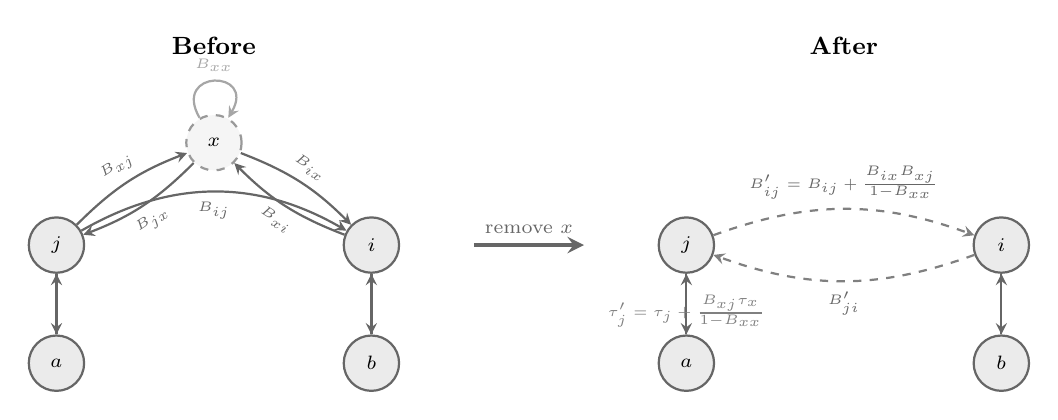
\begin{tikzpicture}[>=stealth, font=\small,
      kept/.style={circle, draw=black!60, fill=black!8, thick,
                   minimum size=20pt, font=\scriptsize},
      removed/.style={circle, draw=black!40, fill=black!4, thick,
                      dashed, minimum size=20pt, font=\scriptsize},
      newedge/.style={->, thick, black!50, dashed},
    ]

    % Left: Before removal
    \begin{scope}[xshift=0cm]
      \node[font=\small\bfseries, anchor=south] at (2.0, 3.8) {Before};

      \node[kept] (j) at (0, 1.5) {$j$};
      \node[removed] (x) at (2, 2.8) {$x$};
      \node[kept] (i) at (4, 1.5) {$i$};
      \node[kept] (a) at (0, 0) {$a$};
      \node[kept] (b) at (4, 0) {$b$};

      % Edges through x
      \draw[->, thick, black!60, bend left=12]
        (j) to node[above, font=\tiny, sloped] {$B_{xj}$} (x);
      \draw[->, thick, black!60, bend left=12]
        (x) to node[below, font=\tiny, sloped] {$B_{jx}$} (j);
      \draw[->, thick, black!60, bend left=12]
        (x) to node[above, font=\tiny, sloped] {$B_{ix}$} (i);
      \draw[->, thick, black!60, bend left=12]
        (i) to node[below, font=\tiny, sloped] {$B_{xi}$} (x);

      % Self-loop on x
      \draw[->, thick, black!35, looseness=5]
        (x) to[out=120, in=60] node[above, font=\tiny] {$B_{xx}$} (x);

      % Other kept edges
      \draw[->, thick, black!60] (j) -- (a);
      \draw[->, thick, black!60] (a) -- (j);
      \draw[->, thick, black!60] (i) -- (b);
      \draw[->, thick, black!60] (b) -- (i);

      % Direct j-i edge (possibly zero)
      \draw[->, thick, black!60, bend left=30]
        (j) to node[below, font=\tiny] {$B_{ij}$} (i);
    \end{scope}

    % Arrow
    \draw[->, ultra thick, black!60] (5.3, 1.5) -- (6.7, 1.5)
      node[midway, above, font=\scriptsize] {remove $x$};

    % Right: After removal
    \begin{scope}[xshift=8cm]
      \node[font=\small\bfseries, anchor=south] at (2.0, 3.8) {After};

      \node[kept] (j2) at (0, 1.5) {$j$};
      \node[kept] (i2) at (4, 1.5) {$i$};
      \node[kept] (a2) at (0, 0) {$a$};
      \node[kept] (b2) at (4, 0) {$b$};

      % Renormalized direct edge (dashed)
      \draw[newedge, bend left=20]
        (j2) to node[above, font=\tiny, text=black!60]
        {$B'_{ij} = B_{ij} + \frac{B_{ix} B_{xj}}{1-B_{xx}}$} (i2);
      \draw[newedge, bend left=20]
        (i2) to node[below, font=\tiny, text=black!60]
        {$B'_{ji}$} (j2);

      % Other kept edges unchanged
      \draw[->, thick, black!60] (j2) -- (a2);
      \draw[->, thick, black!60] (a2) -- (j2);
      \draw[->, thick, black!60] (i2) -- (b2);
      \draw[->, thick, black!60] (b2) -- (i2);

      % Annotation for tau
      \node[font=\tiny, gray, below=4pt] at (j2.south) {$\tau'_j = \tau_j + \frac{B_{xj}\tau_x}{1-B_{xx}}$};
    \end{scope}

  \end{tikzpicture}
  \caption{Graph transformation: removing an intermediate node $x$ (dashed circle). Left: the original network contains five nodes; $x$ is connected to kept nodes $j$ and $i$ with branching probabilities, and may revisit itself. Right: after removing $x$, the branching probabilities and waiting times are renormalized (dashed edges) so that the effective $j \to i$ connection absorbs all paths previously routing through $x$, preserving all MFPTs between kept states exactly.}
  \label{fig:graph-transformation}
\end{figure}


\subsection{Validation of Coarse-Graining}\label{subsec:gt-validation}

Agreement between coarse-grained and microscopic MFPTs serves as the primary validation
criterion for graph transformation. For each retained set and temperature, we compute
$\mathrm{MFPT}_{A \to B}$ and $\mathrm{MFPT}_{B \to A}$ on both the full microscopic
generator $Q$ and the reduced generator $Q^{\mathrm{eff}}$. We run MFPT calculations
on both the coarse and microscopic models and report the collected MFPTs in a summary
table in the Appendix for comparison. Numerical differences are typically less than one
percent, confirming that the GT procedure preserves the kinetic content of the
microscopic model while dramatically reducing dimensionality.

In implementation, each reduced model is written to a
\texttt{GT\_kept\_T\{T\}K/} subdirectory containing $Q^{\mathrm{eff}}(T)$,
$B^{\mathrm{eff}}(T)$, $\boldsymbol{\tau}^{\mathrm{eff}}(T)$,
$\boldsymbol{\pi}^{\mathrm{eff}}(T)$, and the mapping from microscopic indices to
retained indices.


%% ====================================================================
%%  SECTION 6: GRAPH-THEORETIC FEATURE EXTRACTION
%% ====================================================================

\section{Graph-Theoretic Feature Extraction}\label{sec:features}

With the coarse-grained generator $Q^{\mathrm{eff}}$ in hand, we extract a
comprehensive set of graph-theoretic and kinetic features that characterize the KTN
structure and its connection to dynamics.

\subsection{Distance-Based Descriptors}\label{subsec:distances}

\subsubsection{Barrier-based distances}

For each pair of minima $(i,j)$ connected by one or more transition states, we define
the effective barrier height as
\begin{equation}\label{eq:barrier}
  \Delta E_{ij}
  \;=\;
  \min_{\alpha \in \mathcal{S}(i,j)}
  \left[ E_\alpha^\ddagger - \min(E_i, E_j) \right],
\end{equation}
where $\mathcal{S}(i,j)$ is the set of all transition states connecting $i$ and $j$.
This quantity measures the minimum energy rise above the lower of the two minima
needed to transition from one to the other.

Treating $\Delta E_{ij}$ as an edge weight in an undirected graph, we use Dijkstra's
algorithm to compute the shortest-path barrier distance:
\begin{equation}\label{eq:dijkstra}
  d^{\mathrm{barrier}}_{ij}
  \;=\;
  \min_{\text{paths } i \to j}
  \sum_{(a,b) \in \text{path}} \Delta E_{ab}.
\end{equation}

Intuitively, $d^{\mathrm{barrier}}_{ij}$ quantifies the lowest total barrier ``cost''
needed to proceed from minimum $i$ to minimum $j$. For sets of minima, we define
\begin{equation}
  d^{\mathrm{barrier}}_{AB}
  \;=\;
  \min_{i \in A, j \in B} d^{\mathrm{barrier}}_{ij},
\end{equation}
which is a structural measure of how ``far apart'' $A$ and $B$ are on the energy
landscape, independent of vibrational prefactors.

\subsubsection{Rate-based distances}

In addition to barrier heights, the TST rates themselves define a kinetic notion of
distance. For each directed edge $j \to i$ with nonzero rate $k_{i \leftarrow j}$, we
define the logarithmic length:
\begin{equation}\label{eq:log-length}
  \ell_{ij} = -\ln k_{i \leftarrow j}.
\end{equation}

Large rates correspond to small lengths (favorable transitions), and small rates
correspond to large lengths (unfavorable transitions), mirroring the use of negative
log-probabilities in information theory and statistics. On this weighted directed graph,
we apply Dijkstra's algorithm to compute
\begin{equation}
  d^{-\ln k}_{ij}
  \;=\;
  \min_{\text{paths } j \to i}
  \sum_{(a \leftarrow b) \in \text{path}} \ell_{ab}.
\end{equation}

This quantity is a purely kinetic measure of separation that incorporates both
energetic barriers and vibrational prefactors. For sets:
\begin{equation}
  d^{-\ln k}_{AB}
  \;=\;
  \min_{j \in A, i \in B} d^{-\ln k}_{ji}.
\end{equation}

\subsection{Spectral Descriptors}\label{subsec:spectral}

The spectrum of the generator matrix $Q^{\mathrm{eff}}$ provides several
dimensionless descriptors of network structure.

\subsubsection{Spectral gap}

The \emph{spectral gap} is the magnitude of the second eigenvalue:
\begin{equation}
  \gamma = |\lambda_2|.
\end{equation}
A large spectral gap corresponds to fast relaxation to equilibrium, while a small gap
indicates slow equilibration. The spectral gap is directly related to the slowest
relaxation time: $t_2 = 1/\gamma$.

\subsubsection{Spectral gap ratio}

The ratio of the first two nonzero eigenvalues reveals the separation of timescales:
\begin{equation}
  r_{\mathrm{gap}} = \frac{|\lambda_2|}{|\lambda_3|}.
\end{equation}
A large ratio indicates that one slow process dominates over all others, typical of
landscapes with a single rate-limiting barrier. A ratio close to one indicates multiple
competing slow processes, characteristic of multi-funnel landscapes.

\subsubsection{Spectral entropy}

To quantify the complexity of the eigenvalue spectrum, we compute the Shannon entropy
of the normalized eigenvalue magnitudes:
\begin{equation}
  S_{\mathrm{spec}} = -\sum_{k=2}^{N} p_k \ln p_k, \quad \text{where} \quad p_k = \frac{|\lambda_k|}{\sum_{m=2}^{N} |\lambda_m|}.
\end{equation}
A low spectral entropy indicates that one or a few slow modes dominate (a funnel-like
landscape), while high spectral entropy indicates many modes of comparable importance
(a frustrated or multi-funnel landscape).

\subsubsection{Ramanujan score}

Ramanujan graphs are $d$-regular graphs whose nontrivial adjacency eigenvalues satisfy a
specific bound related to the degree and spectral properties
\cite{Lubotzky1988Ramanujan,Murty2003RamanujanSurvey}. The Ramanujan score for a KTN
is a measure of how close the spectral properties approach the Ramanujan bound for
graphs of the same degree. High Ramanujan scores indicate efficient, well-connected
networks whose spectral properties approach theoretical optimality
\cite{Venkatasubramanian2017Teleodynamics}. Networks with high Ramanujan scores tend
to have efficient bottleneck structures and well-separated timescale hierarchies.


\subsection{Network Topology Descriptors}\label{subsec:topology}

Beyond barrier distances and spectral properties, we extract several classical network
measures from each KTN.

Betweenness centrality measures how often a node lies on the shortest paths between
other nodes; nodes with high betweenness are critical for maintaining connectivity
\cite{Newman2006Modularity}. We compute betweenness centrality on both the
barrier-weighted and rate-weighted graphs. Closeness centrality measures the average
distance of a node to all other nodes; central nodes have low closeness. This reveals
which minima are most ``central'' to the network structure.

Community detection algorithms (e.g., the Louvain method) partition the network into
groups of densely connected nodes separated by sparser edges. The number of detected
communities and their sizes reflect the funnel structure of the landscape: single-funnel
landscapes have one large community, while multi-funnel landscapes show multiple
distinct communities.

We also compute the average node degree, degree distribution skewness, and assortativity
(whether high-degree nodes tend to connect to other high-degree nodes). These measures
characterize whether the network has a uniform, hub-like, or heterogeneous structure.


\subsection{Sequence Composition Features}\label{subsec:sequence-features}

In addition to network properties, we include features derived directly from the
peptide sequence: hydropathy index (sum and distribution of hydrophobic character
across the sequence), charge properties (net charge, charge distribution, positive and
negative residue fractions), aromatic content (fraction of aromatic residues like Phe,
Tyr, Trp), and secondary-structure propensities computed from the sequence alone.
These sequence features are included in the feature set to allow the regression models
to exploit any intrinsic sequence biases that correlate with kinetic observables.


\subsection{Connecting Graph Distances to Kinetics}\label{subsec:connecting}

A central aim of this thesis is to compare the structural graph metrics
$d^{\mathrm{barrier}}_{AB}$ and $d^{-\ln k}_{AB}$ with kinetic quantities such as the
forward MFPT ($\mathrm{MFPT}_{A\to B}$), the backward MFPT ($\mathrm{MFPT}_{B\to A}$),
and slow relaxation times ($t_2, t_3, \ldots$) from the eigenvalues of
$Q^{\mathrm{eff}}$.

Hypothetically, if transitions were strongly dominated by a single bottleneck barrier,
we would expect
\begin{equation}
  \log \left( \mathrm{MFPT}_{A\to B} \right)
  \approx \beta \,\Delta E^{\ddagger}_{\mathrm{eff}} + \text{const.}
\end{equation}
for some effective barrier $\Delta E^{\ddagger}_{\mathrm{eff}}$. In a multi-pathway
network, the situation is more complex, but we can still ask empirically: does
$\log \mathrm{MFPT}_{A\to B}$ correlate more strongly with
$d^{\mathrm{barrier}}_{AB}$ or with $d^{-\ln k}_{AB}$? How do these relationships
vary across sequences with different landscape topologies? By computing these
quantities for every sequence and collecting them into a global summary table, we can
perform regression and correlation analyses that connect microscopic landscape structure
to macroscopic kinetics.


%% ====================================================================
%%  SECTION 7: REGRESSION ANALYSIS
%% ====================================================================

\section{Regression Analysis}\label{sec:regression}

With a comprehensive feature set extracted from each coarse-grained KTN, we employ
supervised learning to predict kinetic observables from network properties. This
regression analysis follows in the tradition of quantitative structure-property
relationship (QSPR) modelling in chemical engineering
\cite{Cherkasov2014QSAR,Todeschini2000MolDescriptors,Venkatasubramanian2003QSPR},
adapted here to the specific setting of energy-landscape descriptors as molecular
features and kinetic observables as target properties.


\subsection{Target Variables}\label{subsec:targets}

The primary kinetic observables of interest are:

\begin{itemize}
  \item $\log \mathrm{MFPT}_{A \to B}$: the logarithm of the mean first-passage time
        from the reactant basin to the product basin, quantifying the timescale of
        forward transitions.
  \item $\log \mathrm{MFPT}_{B \to A}$: the backward first-passage time, quantifying
        the timescale of returns.
  \item $\log t_2$: the logarithm of the slowest relaxation time from the generator
        spectrum, reflecting the long-time equilibration timescale.
\end{itemize}

Logarithmic transformation is used because TST rates and kinetic timescales span many
orders of magnitude due to exponential Boltzmann factors. Predicting logarithmic targets
ensures that the regression models assign equal importance across different timescale
ranges.


\subsection{Feature Set Summary}\label{subsec:feature-summary}

The feature set comprises approximately 65 features:

\begin{itemize}
  \item \textbf{Distance-based features} (4): barrier distance $d^{\mathrm{barrier}}_{AB}$,
        rate distance $d^{-\ln k}_{AB}$, and directional variants.
  \item \textbf{Spectral features} (4): spectral gap, gap ratio, spectral entropy,
        Ramanujan score.
  \item \textbf{Centrality features} (8): betweenness and closeness centrality of nodes
        in $A$ and $B$, and network-wide averages.
  \item \textbf{Topology features} (6): average degree, degree distribution skewness,
        assortativity, number of communities, sizes of the largest two communities.
  \item \textbf{Sequence composition features} (8): hydropathy index, charge density,
        aromatic content, secondary-structure propensity, and variants.
  \item \textbf{Transition rate features} (10): summary statistics (mean, median,
        standard deviation, minimum, maximum) of the transition rates in the network.
  \item \textbf{Waiting time features} (8): summary statistics of waiting times at
        retained minima.
  \item \textbf{Barrier statistics} (10): summary statistics of barrier heights across
        all edges.
  \item \textbf{Higher-order features} (7): interactions, polynomial expansions, and
        derived quantities.
\end{itemize}

The features collectively capture the energetic landscape structure, the kinetic
connectivity, the topological organization, and the sequence properties of each peptide.


\subsection{Regression Models}\label{subsec:models}

We train several standard regression models to predict kinetic observables from the
feature set. These span a range from fully interpretable linear methods to flexible
nonlinear ensembles:

\begin{enumerate}
  \item \textbf{Ordinary Least Squares (OLS):} Linear regression with no
        regularization, providing a baseline and interpretable coefficients
        \cite{HastieTibshirani2009ESL}.

  \item \textbf{Ridge Regression:} L2-regularized linear regression ($\alpha$ tuned via
        cross-validation), reducing overfitting for correlated features by shrinking all
        coefficients toward zero \cite{HoerlKennard1970Ridge}.

  \item \textbf{Lasso Regression:} L1-regularized linear regression ($\alpha$ tuned via
        cross-validation), performing automatic feature selection by driving small
        coefficients exactly to zero \cite{Tibshirani1996Lasso}.

  \item \textbf{ElasticNet:} Combined L1 and L2 regularization, balancing sparsity and
        coefficient shrinkage, which is particularly effective when features are
        correlated \cite{ZouHastie2005ElasticNet}.

  \item \textbf{Random Forest:} An ensemble of decision trees, capturing nonlinear
        relationships and feature interactions without explicit feature engineering
        \cite{Breiman2001RandomForests}.

  \item \textbf{Gradient Boosting:} Sequential ensemble of shallow trees, often
        achieving high predictive accuracy and providing feature importance rankings
        \cite{Friedman2001GBM}.
\end{enumerate}

For each model type, hyperparameters (e.g., regularization strength, tree depth,
learning rate) are tuned via cross-validation.


\subsection{Leave-One-Out Cross-Validation}\label{subsec:loocv}

Model performance is evaluated using leave-one-out cross-validation (LOO-CV). For
each of the $M$ sequences in the dataset, we remove the sequence from the training set
(leaving $M-1$ sequences), train each regression model on the remaining data, predict
the kinetic observable for the held-out sequence, and record the prediction error.

LOO-CV provides an unbiased estimate of prediction error on unseen data and is
appropriate for datasets with limited size (typically $M \sim 30$--100 sequences). The
root mean square error (RMSE) and mean absolute error (MAE) on log-transformed targets
are reported as the primary accuracy metrics.


\subsection{Feature Importance and Selection}\label{subsec:importance}

For tree-based models (Random Forest and Gradient Boosting), feature importance is
computed as the decrease in impurity (or loss) when splitting on each feature, averaged
across all trees. We supplement this with permutation importance, which measures the
increase in prediction error when a single feature is randomly shuffled. Features are
ranked by importance, and a cumulative importance plot shows how many features are needed
to explain a given fraction (e.g., 80 percent) of the total variance.

Linear models (OLS, Ridge, Lasso) yield direct coefficients; the magnitude and sign of
each coefficient indicate the direction and strength of its relationship with the target.
The Lasso model is particularly informative because it naturally selects a sparse subset
of features.

Feature importance rankings guide interpretation: features with high importance are more
informative for predicting kinetic observables, providing insight into which network
properties most strongly correlate with dynamics.


\begin{figure}[ht]
  \centering
  \begin{tikzpicture}[
    boxStyle/.style={
      rectangle,
      rounded corners=3pt,
      draw=black!50,
      fill=black!8,
      line width=0.8pt,
      align=center,
      inner sep=6pt,
      minimum height=8mm,
      font=\small,
      text=black
    },
    arrowStyle/.style={
      ->,
      line width=0.8pt,
      black!50
    }
  ]

    % Input: KTNs
    \node[boxStyle, minimum width=3.5cm] (input) at (0, 0)
      {Coarse-grained KTNs\\(all sequences)};

    % Feature Extraction
    \node[boxStyle, minimum width=3.5cm] (features) at (0, -1.2)
      {Feature Extraction\\(65 features)};
    \draw[arrowStyle] (input) -- (features);

    % Feature Box
    \node[boxStyle, minimum width=3.5cm, draw=black!30, fill=black!4] (featlist) at (0, -2.2) {
      \footnotesize
      Distances, Spectral, \\
      Centrality, Topology, \\
      Sequence, Rates
    };
    \draw[arrowStyle, black!30] (features) -- (featlist);

    % Training / Validation Split
    \node[boxStyle, minimum width=3.5cm] (split) at (0, -3.2)
      {LOO Cross-Validation\\(Leave-one-out)};
    \draw[arrowStyle] (featlist) -- (split);

    % Train Models
    \node[boxStyle, minimum width=3.5cm] (models) at (0, -4.4) {Regression Models};
    \draw[arrowStyle] (split) -- (models);

    % Model List
    \node[boxStyle, minimum width=3.5cm, draw=black!30, fill=black!4] (modellist) at (0, -5.6) {
      \footnotesize
      OLS, Ridge, Lasso, \\
      ElasticNet, \\
      Random Forest, Gradient Boosting
    };
    \draw[arrowStyle, black!30] (models) -- (modellist);

    % Output: Predictions
    \node[boxStyle, minimum width=3.5cm] (output) at (0, -6.6)
      {Predictions \\(RMSE, MAE)};
    \draw[arrowStyle] (modellist) -- (output);

    % Right side: Feature Importance
    \node[boxStyle, minimum width=3.5cm, right=1.5cm of features] (importance)
      {Feature Importance};
    \draw[arrowStyle, black!30] (models) -| (importance);
    \node[boxStyle, minimum width=3.5cm, right=1.5cm of featlist, draw=black!30, fill=black!4] (implist) {
      \footnotesize
      Ranked features:\\
      Distance, Spectral, \\
      Centrality, \ldots
    };
    \draw[arrowStyle, black!30] (importance) -- (implist);

  \end{tikzpicture}
  \caption{Regression pipeline for predicting kinetic observables from graph-theoretic features. Coarse-grained KTNs for all sequences are processed to extract 65 features spanning distances, spectral properties, centrality, network topology, and sequence composition. Leave-one-out cross-validation trains each of six regression model types (OLS, Ridge, Lasso, ElasticNet, Random Forest, Gradient Boosting), yielding predictions of $\log$ MFPT and relaxation times. Feature importance rankings from tree-based models identify the most informative network properties.}
  \label{fig:regression-pipeline}
\end{figure}


%% ====================================================================
%%  SECTION 8: SUMMARY
%% ====================================================================

\section{Summary}\label{sec:methods-summary}

This chapter has presented the integrated framework used throughout the thesis:

\begin{enumerate}
  \item \textbf{Energy landscape sampling:} Using the Mpipi potential and
        basin-hopping/discrete path sampling, we build stationary-point databases for
        each hexapeptide sequence.

  \item \textbf{Kinetic Markov models:} Harmonic TST assigns rate constants to
        transitions, yielding a continuous-time Markov chain on minima characterized by
        a generator matrix $Q$, branching probabilities $B$, waiting times
        $\boldsymbol{\tau}$, and stationary distribution $\boldsymbol{\pi}$.

  \item \textbf{Coarse-graining:} Graph transformation eliminates intermediate minima
        while preserving MFPTs between retained states, yielding an effective generator
        $Q^{\mathrm{eff}}$ that is numerically stable and physically interpretable.

  \item \textbf{Feature extraction:} From each coarse-grained KTN, approximately 65
        features are computed, spanning distance-based descriptors, spectral properties,
        centrality measures, network topology, and sequence composition.

  \item \textbf{Regression modelling:} Supervised learning (OLS, Ridge, Lasso,
        ElasticNet, Random Forest, Gradient Boosting) is applied to predict kinetic
        observables ($\log$ MFPT, $\log$ relaxation times) from the feature set, with
        performance evaluated via leave-one-out cross-validation.

  \item \textbf{Validation:} Agreement between microscopic and coarse-grained MFPTs
        confirms the fidelity of the GT reduction, ensuring that kinetic information is
        preserved and results are reliable.
\end{enumerate}

The detailed integration of these methods enables systematic characterization of how
energy landscape structure, network topology, and sequence properties correlate with the
dynamical behavior of hexapeptides.
